% Created 2022-04-28 Thu 20:22
% Intended LaTeX compiler: pdflatex
\documentclass[11pt]{article}
\usepackage[utf8]{inputenc}
\usepackage[T1]{fontenc}
\usepackage{graphicx}
\usepackage{longtable}
\usepackage{wrapfig}
\usepackage{rotating}
\usepackage[normalem]{ulem}
\usepackage{amsmath}
\usepackage{amssymb}
\usepackage{capt-of}
\usepackage{hyperref}
\author{Ali, Mihir, Noah}
\date{\today}
\title{Einführung in die Theoretische Informatik Zusammenfassung}
\hypersetup{
 pdfauthor={Ali, Mihir, Noah},
 pdftitle={Einführung in die Theoretische Informatik Zusammenfassung},
 pdfkeywords={},
 pdfsubject={},
 pdfcreator={Emacs 28.1 (Org mode 9.6)}, 
 pdflang={English}}
\begin{document}

\maketitle
\tableofcontents


\section{Formale Sprachen}
\label{sec:orgc6db29b}

\subsection{Grundbegriffe}
\label{sec:org25b5075}
\begin{itemize}
\item Alphabet \(\Sigma\) (endliche Menge) z.B. \(\{1,0\}\)
\item Wort/String über \(\Sigma\) ist eine endliche Folge von Zeichen aus \(\Sigma\)
\item \(|w|\) länge des Wortes \(w\)
\item Leeres Wort \(\epsilon\)
\item \(uv\) konkatenation der Wörter \(u\) und \(w\)
\item Ist \(w\) ein Wort so ist \(w^0 = \epsilon\) und \(w^{n+1} = ww^n\)
\item \(\Sigma^*\) Menge aller Wörter über \(\Sigma\)
\item (formale) Sprache \(L \subseteq \Sigma^*\)
\end{itemize}

\subsubsection{Operationen auf Sprachen}
\label{sec:org5ffe35f}
Seien \(A,B \subseteq \Sigma^*\)
\begin{itemize}
\item Konkatenation:
\end{itemize}
\(AB = \{uv | u \in A \land v \in B \}\)
\begin{itemize}
\item Konkatenation mit sich selbst:
\end{itemize}
\(A^n = \{w_1 ... w_n | w_1, ... , w_n \in A\} = A ... A\)
\begin{itemize}
\item \(A^* = \{w_1...w_n | n \geq 0 \land w_1, ... , w_n \in A\} = \bigcup_{n\in \mathbb{N}} A^n\)
\item \(A^+ = AA^* = \bigcup_{n \geq 1} A^n\)
\end{itemize}
\begin{enumerate}
\item Sonderfälle:
\label{sec:org8915606}
\begin{itemize}
\item \(\forall A: \epsilon \in A^*\)
\item \(\emptyset^* = \{\epsilon\}\)
\item \(\emptyset A = \emptyset\)
\item \(\{\epsilon \} A = A\)
\item \(A^*A^* = A^* = (A^*)^*\)
\end{itemize}
\end{enumerate}

\subsubsection{Grammatiken}
\label{sec:org4a269cc}
4-Tupel \(G = (V,\Sigma,P,S)\)
\begin{itemize}
\item \(V\) ist endliche Menge von Nichtterminalzeichen
\item \(\Sigma\) ist endliche Menga von Terminalzeichen (= Alphabet)
\item \(P \subseteq (V \cup \Sigma)^* \times (V \cup \Sigma)^*\) ist Menge von Produktionen
\item \(S \in V\) ist das Startsymbol
\end{itemize}

Die Sprache von G ist die Menge aller Wörter, die von G erzeugt werden. Sie wird mit \(L(G)\) bezeichnet.
Also jedes Wort, dass die Grammatik erzeugt muss in der Sprache erhalten sein und jedes Wort in der Sprache muss von der Grammatik erzeugt werden.
\begin{enumerate}
\item Reflexve transitive Hülle
\label{sec:orga055a3e}

\begin{itemize}
\item \(\alpha \rightarrow^0_G \alpha\)
\item \(\alpha \rightarrow^{n+1}_G \gamma: \exists \beta. \alpha \rightarrow^n_G \rightarrow_G \gamma\)
\item \(\alpha \rightarrow^{*}_G \beta : \exists n. \alpha \rightarrow^n_G \beta\)
\item \(\alpha \rightarrow^{+}_G \beta: \exists n>0. \alpha \rightarrow^n_G \beta\)
\end{itemize}
\end{enumerate}

\subsubsection{Chomsky Hierarchie}
\label{sec:org04cf022}
Eine Grammatik G ist vom
\begin{itemize}
\item Typ 0 immer
\item Typ 1 falls fpr jede Produktion \(\alpha \rightarrow \beta\) außer \(S \rightarrow \epsilon\) gilt \(|\alpha| \leq |\beta|\)
\item Typ 2 Falls G vom typ 1 ist und für jede Produktion \(\alpha \righarrow \beta\) gilt \(\alpha \in V\)
\item Typ 3 falls G vom Typ 2 ist und für jede Produktion \(\alpha \rightarrow \beta\) außer \(S \rightarrow \epsilon\) gilt \(\beta \in \Sigma \cup \Sigma V\)
\end{itemize}

\begin{enumerate}
\item Grmmatiken und Sprachklassen:
\label{sec:org607f946}
\begin{center}
\begin{tabular}{lll}
Typ 3 & Rechtslineare Grammatiken & Reguläre Sprachen\\
Typ 2 & Kontextfreie Grammatik & Kontextfreie Sprachen\\
Typ 1 & Kontextsensitive Grammatik & Kontextsens. Sprachen\\
Typ 0 & Phrasenstrukturgrammatik & Rekursiv aufzählbare Sprachen\\
\end{tabular}
\end{center}

\item Satz 2.13
\label{sec:org6f45341}
\(L(Typ 3) \subset L(Typ 2) \subset L(Typ 1) \subset L(Typ 0)\)
\end{enumerate}

\subsubsection{Wortproblem}
\label{sec:org2f30a22}
Gegeben: eine Grammatik G, ein Wort \(w \in \Sigma^*\)
Frage: Ist das Wort in w enthalten (\(w \in L(G)\))?

\section{Reguläre Sprachen}
\label{sec:orgc1be568}

\begin{figure}[htbp]
\centering
\includegraphics[width=.9\linewidth]{./img/2-kapitel/reguläre_sprachen.png}
\caption{Reguläre Sprachen Schema}
\end{figure}

\subsection{Deterministische endliche Automaten}
\label{sec:org44185a7}
\begin{figure}[htbp]
\centering
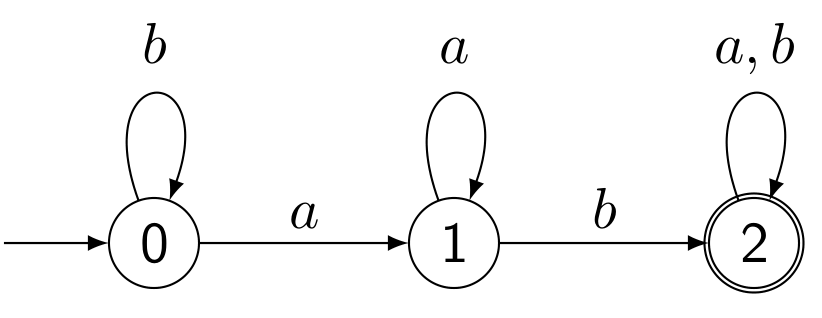
\includegraphics[width=.9\linewidth]{./img/2-kapitel/automat_bsp.png}
\caption{Beispiel Automat}
\end{figure}

\begin{itemize}
\item Beispiel:
\begin{itemize}
\item Eingabewort \(baba \rightarrow\) Zustandsfolge 0,0,1,2,2
\end{itemize}
\item ``Bei dieser Grammatik muss mindestens nach einem a ein b kommen''
\item Die Sprache des DFA ist die Menge aller Wörter über \(\{a,b\}\), die ab enthalten
\end{itemize}

Erkannte Sprache: Menge der Wörter, die vom Startzustand in einen Endzustand führen.
Recognizer, die nur einmal das Wort durchläuft und in linearer Zeit es akzeptiert oder ablehnt.

\subsubsection{Definition}
\label{sec:orgad09e98}
Ein deterministischer endlicher Automat \(M = (Q,\Sigma, \delta, q_0, F)\) besteht aus
\begin{itemize}
\item endliche Menge von Zuständen Q
\item endlichem Eingabealphabet \(\Sigma\)
\item einer totalen Übergangsfunktion \(\delta: Q \times \Sigma \rightarrow Q\)
\item eienm Startzustand \(q_0 \in Q\)
\item einer Menge \(F \subset Q\) von Endzuständen
\end{itemize}

\subsubsection{Akzeptierte Sprachen (Definition 3.2)}
\label{sec:org178d19b}
Von M akzeptierte Sprache \(L(M) := \{w \in \Sigma^* | \hat{\delta}(q_0, w) \in F\}\) wobei \\
\(\hat{\delta}: Q \times \Sigma^* \rightarrow Q\) induktiv definiert ist: \\
\(\hat{\delta}(q,\epsilon) = q\) \\
\(\hat{\delta}(q,aw) = \hat{\delta}(\delta(q,a),w)\), für \(a \in \Sigma, w \in \Sigma^*\) \\
(\(\hat{\delta}(q, w)\) bezeichnet den Zustand, den man aus \(q\) mit \(w\) erreicht.)\\
Eine Sprache ist regulär \textbf{gdw} sie von einem DFA akzeptiert wird.
\end{document}
